\chapter{Plotluck}

\section{Introduction}

Coined as the ``ggplot2 version of `I'm feeling lucky!''', \texttt{plotluck} is designed to consider the characteristics of a data frame to decide, through a heuristic algorithm, the most appropriate plot to represent the data.
The package has scatter, box, bar, violin, density, heat map, hexagon bin, and spine plots available.
The ultimate goal of the package is to allow users to explore which type of plot would best fit their data, instead of becoming burdened with the creating code in R.

\section{Objectives}
In this assignment, we will use \texttt{plotluck} to explore rapid visualization of several data sets.
The code created is a good place to start, but we encourage you to continue exploring the package.
The website Gapminder has an extreme amount of data sets available for public use, and R has around 30 data sets built in.

\section{Deliverable}
As plot luck is created for finding and forming appropriate graphics for respective data sets, the desired deliverable will be dependent on the data set used.

For example, plots using ggplot2's \texttt{mpg} data set are shown in figures \ref{fig:mpg1}, \ref{fig:mpg2}, and \ref{fig:mpg3}.

\begin{figure}[htbp!]
    \centering
    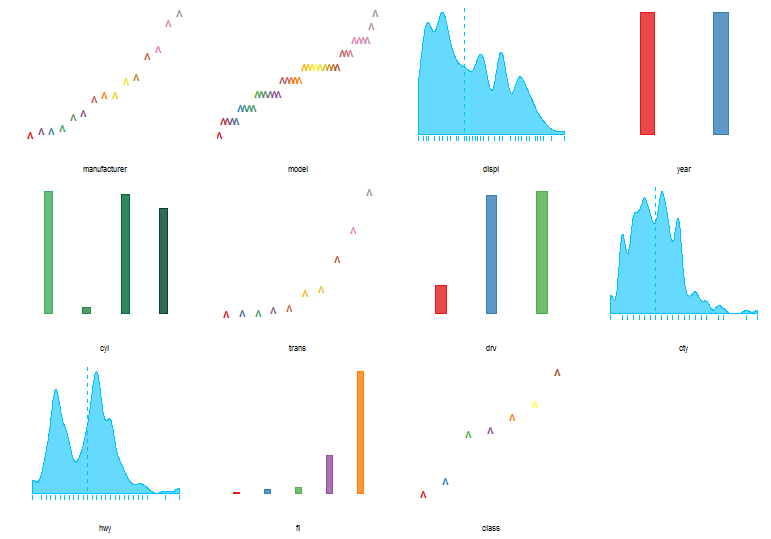
\includegraphics[width=.5\textwidth]{pictures/plotluck/mpgall}
    \caption{Plotting every variable in \texttt{mpg}}
    \label{fig:mpg1}
\end{figure}

\begin{figure}[htbp!]
    \centering
    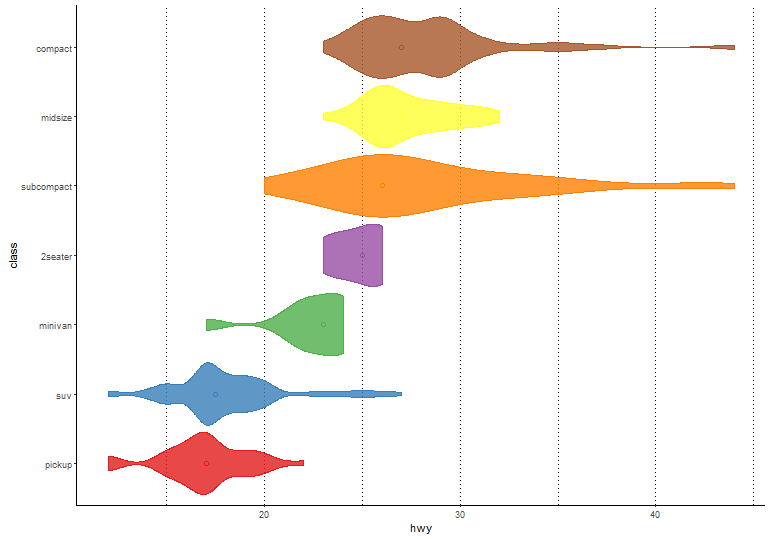
\includegraphics[width=.5\textwidth]{pictures/plotluck/mpg1}
    \caption{Highway mileage to class}
    \label{fig:mpg2}
\end{figure}

\begin{figure}[htbp!]
    \centering
    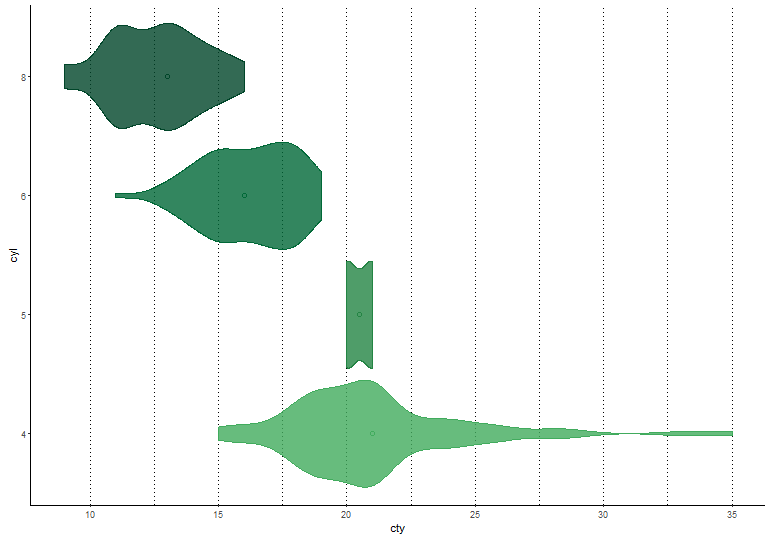
\includegraphics[width=.5\textwidth]{pictures/plotluck/mpg2}
    \caption{Cylinder count vs city mileage}
    \label{fig:mpg3}
\end{figure}

More examples include figures \ref{diamondprice} and \ref{txhousing}.

\begin{figure}[htbp!]
    \centering
    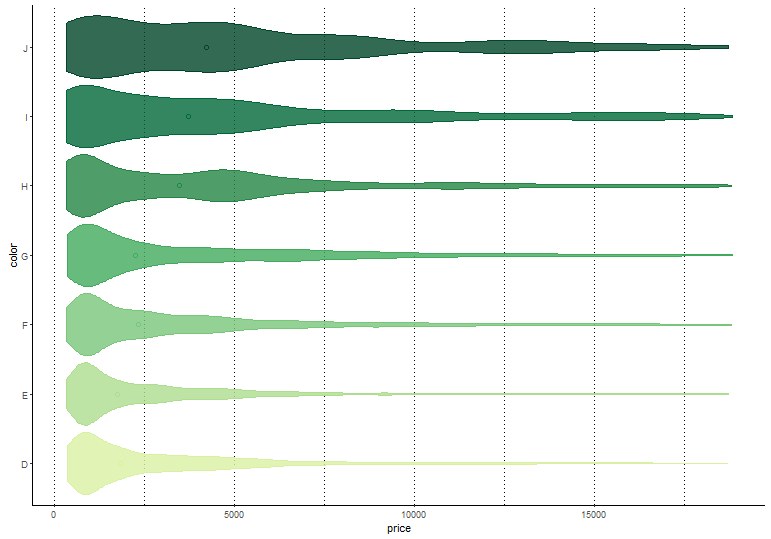
\includegraphics[width=.5\textwidth]{pictures/plotluck/diamonds1}
    \caption{Price to color in the \texttt{diamonds} dataset}
    \label{diamondprice}
\end{figure}

\begin{figure}[htbp!]
    \centering
    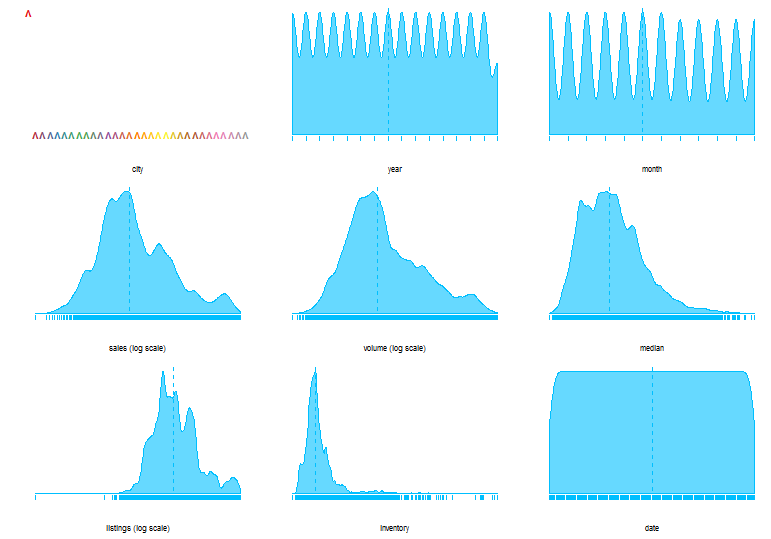
\includegraphics[width=.5\textwidth]{pictures/plotluck/txhousingall}
    \caption{Plotting every variable in \texttt{txhousing}}
    \label{txhousing}
\end{figure}

\section{Teaching Code}
\begin{lstlisting}
# Example for Plotluck

# Clean up and import plotluck
rm(list=ls())
library(plotluck)
setwd("C:/Your/R/Directory")

# Let's work with the faithful data
# What's in this data set?
plotluck(.~1, faithful)

# Look at everything vs everything else:
plotluck(.~., faithful)

# Eruptions look interesting, what can that tell us?
plotluck(eruptions~., faithful)
plotluck(eruptions~waiting, faithful)

# Let's look at airquality
plotluck(.~1, data=airquality)

# We can generate some interesting plots because Month is discrete
plotluck(Temp~Month, airquality)
plotluck(Wind~Month, airquality)
plotluck(Ozone~Month, airquality)

# And some more interesting ones
plotluck(Temp~Solar.R+Ozone, airquality)
plotluck(Temp~Wind+Ozone, airquality)
plotluck(Temp~Solar.R|Month, airquality)

# Let's look at mtcars
# This tells us more about the variables
plotluck(.~1, mtcars)
# Here are some interesting examples
plotluck(vs~gear, mtcars)
plotluck(mpg~wt, mtcars)

# Let's explore random plotting!
data(diamonds, package='ggplot2')
set.seed(100)
# Run this several times to get random plots
sample.plotluck(diamonds)
# Note the following hex plots:
plotluck(depth~x, diamonds)
plotluck(price~carat, diamonds)

\end{lstlisting}

\section{Example Student Code}
\begin{lstlisting}
# EXAMPLE KEY
# Date
# Plotluck Exercises - KEY

# Clean up and import plotluck
rm(list=ls())
library(plotluck)
setwd("D:/School/RCompSci/book/plotluck")

# Using the following command:
# data(dataset_name, package='ggplot2')
# Look at three of the following datasets using plotluck:
# mpg, msleep, diamonds, presidential, txhousing, seals

# Code goes here
\end{lstlisting}

\section{Further Readings}
\begin{enumerate}
    \item \url{https://cran.r-project.org/web/packages/plotluck/index.html}
    \item \url{https://cran.r-project.org/web/packages/plotluck/vignettes/plotluck.html}
\end{enumerate}
